\documentclass[a4paper]{tufte-book}
\setlength\parindent{0em}
\setlength\parskip{1em}
\raggedbottom

%----------%
% SETTINGS %
%----------%

\makeatletter
\def\input@path{{./settings/}}
\makeatother
\usepackage{booktabs}

\usepackage{lipsum}
% \usepackage{import}  % for relative paths importing

% Language-related
\usepackage[english]{babel}
\usepackage[autostyle, german=guillemets, english=american]{csquotes}

% Packages
\usepackage{amsmath, mathtools, bm, commath}
\usepackage{physics}
\usepackage{siunitx}
\usepackage{nicematrix}

% General settings
\allowdisplaybreaks     % Allows for equations to break between pages

% Cancel-lines related
\usepackage[thicklines]{cancel}
\renewcommand\CancelColor{\color{xred}}
\newcommand{\cancelcol}[2][xred]{ % This is such a silly solution...
	\renewcommand\CancelColor{\color{#1}}
	\cancel{#2}
	\renewcommand\CancelColor{\color{xred}}
}

% Easier space-notation
\newcommand{\Rs}[1][]{\mathbb{R}^{#1}}
\newcommand{\Cs}[1][]{\mathbb{C}^{#1}}

% Set notation for vectors (currently: bold letters)
\renewcommand{\vec}[1]{\bm{#1}}
\newcommand{\uvec}[1]{\bm{\hat{#1}}}
\newcommand{\vnorm}[1]{\left\| \vec{#1} \right\|}
\newcommand{\cvec}[1]{\bm{\overline{#1}}}
\newcommand{\mat}[1]{\bm{#1}}

% Vector operations
\newcommand{\inner}[2]{\langle #1,#2 \rangle}

% Dual space related
\newcommand{\dualspace}[1]{#1^{*}}
\newcommand{\dualvec}[1]{\vec{#1}^{*}}

% Row- and column-vectors: arguments separated by ";".
% Example: $\vec{a} = \colvec{1;2;3;4}$.
\makeatletter
\newcommand\rcvector[2][\\]{\ensuremath{%
  \global\def\rc@delim{#1}%
    \negthinspace\begin{bmatrix}
      \rc@vector #2;\relax\noexpand\@eolst%
    \end{bmatrix}}}
\def\rc@vector #1;#2\@eolst{%
  \ifx\relax#2\relax
    #1
  \else
    #1\rc@delim
    \rc@vector #2\@eolst%
  \fi}
\makeatother
\newcommand{\colvec}{\rcvector}
\newcommand{\rowvec}[1]{\rcvector[,\;]{#1}}
\newcommand{\GenericRowVec}[2][n]{\rowvec{#2_{1};#2_{2};\dots;#2_{#1}}}
\newcommand{\GenericColVec}[2][n]{\colvec{#2^{1};#2^{2};\vdots;#2^{#1}}}

% Colored vectors
\newcommand{\colorVec}[2]{\color{#1}{\vec{#2}}\color{black}}
\newcommand{\vred}{\colorVec{xdarkred}{v}}
\newcommand{\vblue}{\colorVec{xdarkblue}{v}}
\newcommand{\vgreen}{\colorVec{xdarkgreen}{v}}

% Basis vectors and transformations
\newcommand{\eb}[1]{\vec{e}_{#1}}
\newcommand{\ebc}[1]{\tilde{\vec{e}}_{#1}}
\newcommand{\ebr}[1]{\color{xdarkblue}\eb{#1}\color{black}}
\newcommand{\ebcr}[1]{\color{xdarkred}\ebc{#1}\color{black}}
\newcommand{\oldB}{\color{xdarkblue}B\color{black}}
\newcommand{\newB}{\color{xdarkred}\tilde{B}\color{black}}
\newcommand{\Forw}{\bm{F}}
\newcommand{\Backw}{\bm{F^{-1}}}

% Dark equal?
\newcommand{\beq}{\color{black}{=}}

% Better imaginary unit and natural base notation (to separate from variables)
\newcommand{\iu}{\mathrm{i}\mkern1mu}
\newcommand{\eu}{\mathrm{e}}
\newcommand{\Eu}[1]{\mathrm{e}^{#1}}
\newcommand{\EX}[1]{\exp\left(#1\right)}

% General nice matrix
\newcommand{\GNMatrix}[3]{
  \begin{bNiceMatrix}
    #1_{11} & #1_{12} & \dots & #1_{1#3}\\
    #1_{21} & #1_{22} & \dots & #1_{2#3}\\
    \vdots & \vdots & \Ddots & \vdots\\
    #1_{#21} & #1_{#22} & \dots & #1_{#2#3}
  \end{bNiceMatrix}
}

% Clever references (tufte-latex clashes with \autoref)
% \usepackage{cleveref}
% \crefname{figure}{Figure}{Figure}
% \crefname{equation}{Equation}{Equation}

% Hyperrefs etc.
\usepackage[compatibility=false]{caption}
\usepackage{hyperref}
\hypersetup{
  colorlinks=true,
  linkcolor=blue,
  filecolor=magenta,      
  urlcolor=cyan,
  pdftitle={Spinors for Beginners},
  pdfauthor={Peleg Bar Sapir},
}

% Packages
\usepackage{xcolor}

%%%%%%%%%%%%%%%%%%%%%%%%
%        COLORS        %
%%%%%%%%%%%%%%%%%%%%%%%%

% Normal colors
\definecolor{xred}{HTML}{BD4242}
\definecolor{xblue}{HTML}{4268BD}
\definecolor{xgreen}{HTML}{52B256}
\definecolor{xpurple}{HTML}{7F52B2}
\definecolor{xorange}{HTML}{FD9337}
\definecolor{xdotted}{HTML}{999999}
\definecolor{xgray}{HTML}{777777}
\definecolor{xcyan}{HTML}{80F5DC}
\definecolor{xpink}{HTML}{F690EA}
\definecolor{xgrayblue}{HTML}{49B095}
\definecolor{xgraycyan}{HTML}{5AA1B9}

% Dark colors
\colorlet{xdarkred}{red!85!black}
\colorlet{xdarkblue}{xblue!85!black}
\colorlet{xdarkgreen}{xgreen!85!black}
\colorlet{xdarkpurple}{xpurple!85!black}
\colorlet{xdarkorange}{xorange!85!black}
\colorlet{xdarkcyan}{xcyan!85!black}

% Very dark colors
\colorlet{xverydarkblue}{xblue!50!black}

% Document-specific colors
\colorlet{normaltextcolor}{black}
\colorlet{figtextcolor}{xblue}

% Enumerated colors
\colorlet{xcol0}{black}
\colorlet{xcol1}{xred}
\colorlet{xcol2}{xblue}
\colorlet{xcol3}{xgreen}
\colorlet{xcol4}{xpurple}
\colorlet{xcol5}{xorange}
\colorlet{xcol6}{xcyan}
\colorlet{xcol7}{xpink!75!black}

%%%%%%%%%%%%%%%%%%%%%
%        PGF        %
%%%%%%%%%%%%%%%%%%%%%

\usepackage{pgfplots}
\usepgfplotslibrary{fillbetween}%, colormaps, colorbrewer, patchplots}
\pgfplotsset{
  compat=1.16,
  %% Styles %%
  xyplane/.style = {
    axis x line=middle,
    axis y line=middle,
    xlabel=$x$,
    ylabel=$y$,
    every axis x label/.style={at={(ticklabel* cs:1.02)}, anchor=west},
    every axis y label/.style={at={(ticklabel* cs:1.02)}, anchor=south},
    axis line style={stealth-stealth, very thick, black!65},
    label style={font=\large},
    tick label style={font=\large},
    samples=100,
    xmin=-5, xmax=5,
    ymin=-5, ymax=5,
    grid=both,
    major grid style={black!15},
    minor grid style={black!10},
    xticklabels={,},
    yticklabels={,},
  },
  xynogrid/.style = {
    xyplane,
    major grid style={opacity=0},
    minor grid style={opacity=0},
  },
  xyempty/.style = {
    xyplane,
    axis line style = {draw=none},
    tick style = {draw=none},
    xlabel = {},
    ylabel = {},
    major grid style = {draw=black!0},
  },
  hyperplane1D/.style = {thick, #1},
  %% Function plots
  function/.style = {
    ultra thick, draw=#1,
  },
  filledfunction/.style = {
    function={#1}, opacity=1, fill=#1, fill opacity=0.3,
  },
}

%%%%%%%%%%%%%%%%%%%%%%
%        TikZ        %
%%%%%%%%%%%%%%%%%%%%%%

\usepackage{tikz, tikz-3dplot}
\usetikzlibrary{calc, shapes, intersections, backgrounds, decorations.markings}
\tikzset{
  %% Styles %%
  vector/.style = {#1, ultra thick, -stealth, cap=round},
  pics/ruler/.style n args = {5}{
      code = {
          % Parameters
          \pgfmathsetmacro{\width}{#1}
          \pgfmathsetmacro{\height}{#2}
          \pgfmathsetmacro{\yMaj}{\height/3}
          \pgfmathsetmacro{\yMid}{\yMaj*0.7}
          \pgfmathsetmacro{\yMin}{\yMaj*0.5}
          \pgfmathsetmacro{\dxMaj}{#3}
          \pgfmathsetmacro{\dxMin}{\dxMaj*0.1}
          \pgfmathsetmacro{\maxMajGrad}{ceil((\width-2)/\dxMaj)}
          \pgfmathsetmacro{\maxMidGrad}{\maxMajGrad-0.5}
          \pgfmathsetmacro{\maxMinGrad}{(\maxMajGrad-1)*10}

          % Main rectangle
          \draw[thick, fill=#4] (0,0) rectangle (\width,\height);

          % Graduations
          % Major
          \foreach \x [count=\k from 0] in {1,2,...,\maxMajGrad}
              \draw[thick] ({\x*\dxMaj}, \height) -- ++(0.0,-\yMaj) node[below] (g\k) {$\k$};
          % Middle
          \foreach \y in {1.5,2.5,...,\maxMidGrad}
              \draw[thick] ({\y*\dxMaj}, \height) -- ++(0.0,-\yMid);
          % Minor
          \foreach \z in {1,2,...,\maxMinGrad} 
              \draw[thin] ({\dxMaj+\z*\dxMin}, \height) -- ++(0.0,-\yMin);

          % units label
          \node[below of=g0, font=\small, yshift={11*\height}] {#5};
      }
  },
  arcnode/.style 2 args={                
    decoration={
      raise=#1,             
      markings,   
      mark=at position 0.5 with { 
        \node[inner sep=0] {#2};
      }
    },
    postaction={decorate}
  },
  perpline/.style = {
    very thick, densely dotted, draw=#1
  }
}
\newcommand{\rulerTwoD}[6]{
  \pgfmathsetmacro{\Vx}{#1};
  \pgfmathsetmacro{\Vy}{#2};
  \pgfmathsetmacro{\a}{#3};
  \pgfmathsetmacro{\scale}{3*\a/sqrt(\Vx*\Vx+\Vy*\Vy)};
  \foreach \b in {-#4,...,#4}
    \addplot[very thick, #5] {-(\Vx/\Vy)*x+(\b/\a)};
}

% section numbering
\setcounter{secnumdepth}{2}

% Chapter title
\titleformat{\chapter}
[block]% shape
{\relax\ifthenelse{\NOT\boolean{@tufte@symmetric}}{\begin{fullwidth}}{}}% format applied to label+text
{\itshape\huge\thechapter}% label
{1em}% horizontal separation between label and title body
{\huge\rmfamily\itshape}% before the title body
[\ifthenelse{\NOT\boolean{@tufte@symmetric}}{\end{fullwidth}}{}]% after the title body


%----------%
% DOCUMENT %
%----------%

\begin{document}
% \part{Tests}
% \chapter{General layout test}
% \section{This is a title}\label{sec:title}
\lipsum[2-2]

\begin{marginfigure}
    \begin{center}
    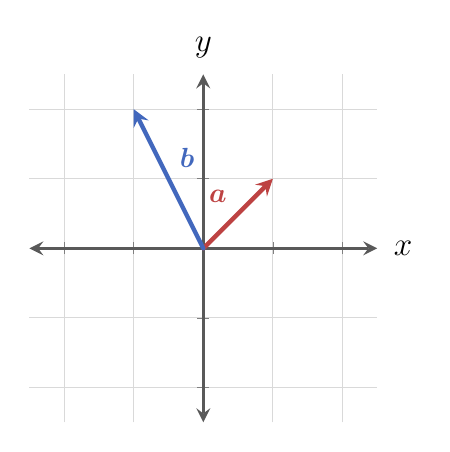
\begin{tikzpicture}
    \begin{axis}[
        xyplane,
        width=6cm, height=6cm,
    ]
        \draw[vector={xred}] (0,0) -- (2,2) node[midway, above left] {$\vec{a}$};
        \draw[vector={xblue}] (0,0) -- (-2,4) node[midway, above right] {$\vec{b}$};
    \end{axis}
    \end{tikzpicture}
    \end{center}
    \caption{A margin figure.}
    \label{fig:margin_figure}
\end{marginfigure}

This is a manualy-typed text. It even points to a figure (see \autoref{fig:margin_figure}).


\makeatletter

%% -- PART 1: Background -- %%
\part{Background Topics}

% Linear algebra
\chapter{Linear Algebra}
\def\input@path{{./parts/background/linear_algebra}}
\section{Preface}
\newthought{The goal of this chapter} is to review a few of the more advanced topics in linear algebra, which are important both for learning the other background topics, as well as the actual topic of spinors.

For example, the topic of dual vectors can help with understanding the what the Dira/bra-ket notation actually means, and cement a deeper understanding of the basic ideas of quantum physics. The topic of absrtact vector spaces provides a good foundation for topics such as geometric- and abstract algebra.

More to be written\ldots

\section{Vectors and Vector Spaces}

\input{linear_transformations}
\input{matrices}
\input{eigenvectors}
\input{quaternions}
\section{Advanced Notation and Einstein's Summation}

\input{further_reading}

% - Geometric algebra
\chapter{Geometric Algebra}
\def\input@path{{./parts/background/geometric_algebra}}
\section{Preface}
\newthought{The goal of this chapter} is to review a few of the more advanced topics in linear algebra, which are important both for learning the other background topics, as well as the actual topic of spinors.

For example, the topic of dual vectors can help with understanding the what the Dira/bra-ket notation actually means, and cement a deeper understanding of the basic ideas of quantum physics. The topic of absrtact vector spaces provides a good foundation for topics such as geometric- and abstract algebra.

More to be written\ldots


% - Abstract algebra
\chapter{Abstract Algebra}
\def\input@path{{./parts/background/abstract_algebra}}
\section{Preface}
\newthought{The goal of this chapter} is to review a few of the more advanced topics in linear algebra, which are important both for learning the other background topics, as well as the actual topic of spinors.

For example, the topic of dual vectors can help with understanding the what the Dira/bra-ket notation actually means, and cement a deeper understanding of the basic ideas of quantum physics. The topic of absrtact vector spaces provides a good foundation for topics such as geometric- and abstract algebra.

More to be written\ldots


% - Lie groups and algebras
\chapter{Lie Groups and Algebras}
\def\input@path{{./parts/background/lie_groups_algebras}}
\section{Preface}
\newthought{The goal of this chapter} is to review a few of the more advanced topics in linear algebra, which are important both for learning the other background topics, as well as the actual topic of spinors.

For example, the topic of dual vectors can help with understanding the what the Dira/bra-ket notation actually means, and cement a deeper understanding of the basic ideas of quantum physics. The topic of absrtact vector spaces provides a good foundation for topics such as geometric- and abstract algebra.

More to be written\ldots


%% -- PART 2: Spinors -- %%
\part{Spinors}


\makeatother
\end{document}
